\section{Estimating the Channel\label{sec:chanEst}}
The first experiment performed had the purpose of estimating the channel properties in different conditions. For this experiment, no dynamic packet length control scheme was used. Instead, simple, out-of-the box packet transmission  with different packet lengths were used. Based on the number of received packages the PRR, $p(l)$, and efficiency, $\mathcal{E}$, have been estimated. Two simple programs are implemented: One for a transmitter mote and one for a receiver mote.
\paragraph{Transmitter} The transmitter sends a fixed number of packets to the receiver. The length of the packets decreases gradually in steps of $10$ bytes. In the specific implementation the transmitter sends $1000$ packets, one every $50$ milliseconds, starting with the maximum packet length $l = 100$. After the first batch of messages are sent, the transmitter waits $5$ seconds before sending the next batch of (smaller) packets.
\paragraph{Receiver} The receiver is slightly less complicated as its only role is to count the number of received messages and to periodically report this counter and the current received payload length $l$ to a computer, using the serial connection. In the current implementation, a serial message is transmitted every $2$ seconds.
\\[8pt]
With the information provided by the receiver, the Packet Reception Rate (PRR) and transmission efficiency, $\mathcal{E}$, are calculated using a \textsc{Python} script. The results for the channel where the distance between the motes was $35$ meters can be seen in figure \ref{fig:35mTest} and for the $45$ meters distance in figure \ref{fig:45mTest}. For the channel with the motes placed $35$ meters apart, it can be seen that the maximum transmission efficiency $\mathcal{E}$ is reached when they payload is about $80$ bytes. Even though the measurements for the channel with a distance between the motes of $45$ meters present a lot of variation, it is possible to see that the efficiency reaches a maximum at a lower packet size $l$ ($50-80$ bytes). This result is expected as the higher distance between the motes deteriorates the quality of the channel and increases the probability of bit error - therefore increasing the probability of corrupting a larger packet.
\\[8pt]
The results presented show the relationship between distance and transmission efficiency of the channel. These results will be used to verify that the DPLC scheme presented in later sections functions as expected, thus choosing the a dynamic packet length that maximizes the throughput in the channel. The comparable results obtained by testing the DPLC scheme are presented in section \ref{sec:schemeTest}.

\begin{figure}
\centering
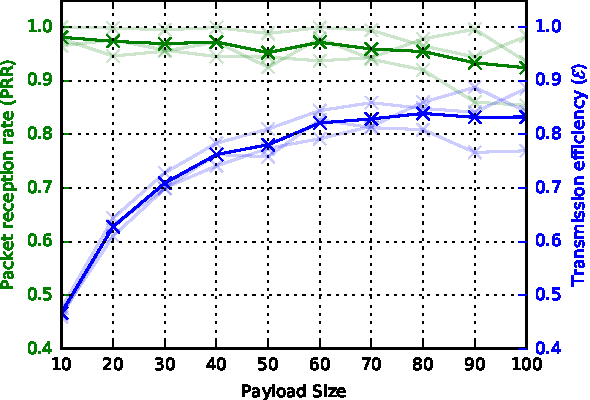
\includegraphics[scale=1]{figs/35mTest.pdf} 
\caption{\textit{PRR and transmission efficiency as a function of payload size, 35 meters apart}\label{fig:35mTest}}
\end{figure}

\begin{figure}
\centering
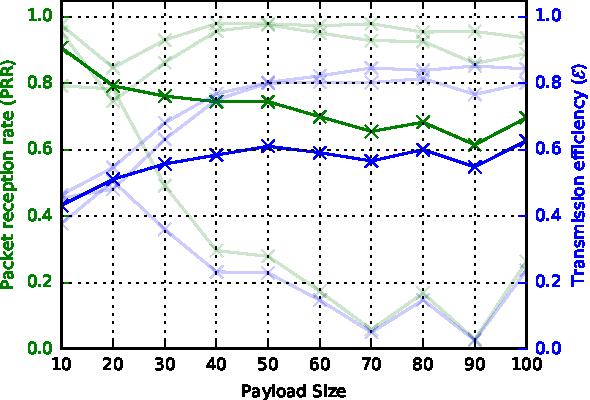
\includegraphics[scale=1]{figs/45mTest.pdf} 
\caption{\textit{PRR and transmission efficiency as a function of payload size, 45 meters apart}\label{fig:45mTest}}
\end{figure}